\chapter{Experiment 1}
\label{cap:experiment1}

\textbf{Author: } 

The first experiment tests whether the trained neural network from Section~\ref{sec:implementation_neural_network} generalises to other objects. Since it is impossible to train the neural network for all existing objects, this experiment tests if the neural network can, by learning from one object, determine the distance to other objects as well.

\section{Setup}
The addition of the third convolutional layer (see Fig.~\ref{pic:implementation_neuralNetwork_modificationsToTheNN_model}) allowed to solve problems of a higher complexity, as compared to before. For this experiment the neural network was further developed to attain a colour image as an input and output the corresponding x-, y- and z-coordinate. These changes dramatically increased the number of parameters and therefore the need for RAM and computation power. 

The best system available at that time was a pc with a NVIDIA 2080 TI, which has 11 GB of VRAM (or "video random access memory"). To also fully take advantage of the cuda cores (parallel processors for graphical computing), the authors decided to use tensorflow with the GPU only. These changes resulted in much greater performance than before (10s to train with ten images on the previous configuration opposed to 32 ms on the current one). One disadvantage of this solution is, that only the GPU is used for computing, which means that only the VRAM can be used. But, since the performance was so much better, it was worth it to lower the batch size from 40 to 20 images at a time, which, after testing, is the optimal value and uses about 10.8 of the 11 GB of VRAM available.

\section{Sequence of Events}
To train the neural network, the authors chose the monkey head object, as depicted in Figure~\ref{pic:implementation_generatingData_testObject}. This neural network is trained exclusively on the monkey head until the mean error is confirmed to be less than 10\%. For training the authors use 500 distinct images each for monkey heads of 5 different sizes, totalling in 2500 images.

After the neural network has been trained and reached a respectable accuracy, the authors will then test the neural network with images of another object. This object can again be seen in Figure~\ref{pic:implementation_generatingData_testObject}. Because we are not training with these images, only 50 images for each of the 5 sizes are evaluated. First the training aspect (changing the weights of the neural network according to the new input) will be disabled, allowing the authors to figure out the accuracy of the neural network when viewing new images for the first time, without changing the neural network itself.

Then the training aspect will be enabled again and the time and effort needed to reach an accuracy of under 15\% when retraining exclusively for the new object with the already pre-trained weights will be measured.

\section{Results}
After training the neural network with the monkey head object, the values predicted by the neural network for the vase object differed from the actual values by the following values for all vase images:

\begin{table}[h!]
	\begin{tabular}{ll|l}
		&     & \textbf{Difference in meters} \\
		\hline
		\textbf{average} & x   & 3.023                         \\
		& y   & 0.443                         \\
		& z   & 3.18                          \\
		& all & 2.215                         \\
		\hline
		\textbf{minimum} & x   & 0.011                         \\
		& y   & 0.011                         \\
		& z   & 2.259                         \\
		\hline
		\textbf{maximum} & x   & 6.577                         \\
		& y   & 1.224                         \\
		& z   & 7.132                                                  
	\end{tabular}
\end{table}

So overall this resulted in an average error of 2.215 meters.

The time needed to train the neural network with the vase images, which resulted in the desired accuracy of more than 85\%, was 40.62 seconds, training with 1220 images of the vase object.


\begin{figure*}[h!]
	\centering
	\begin{subfigure}[t]{\textwidth}
		\centering
		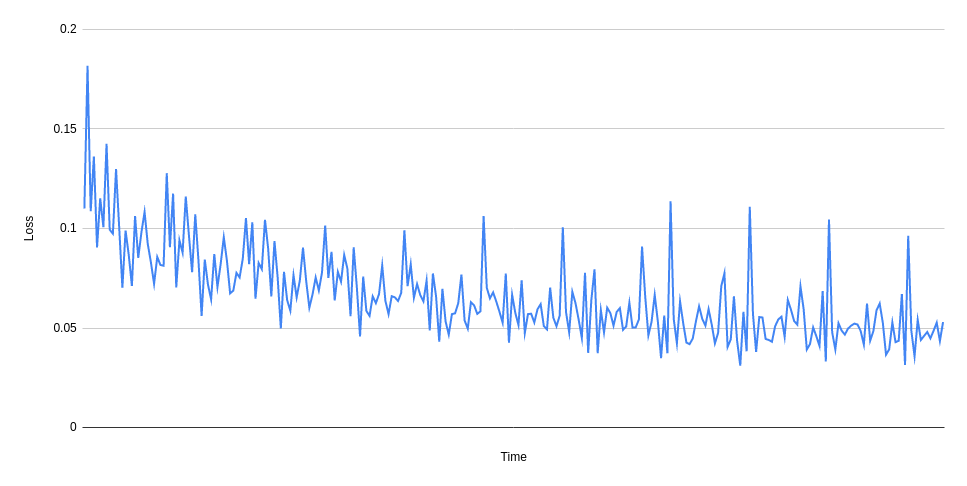
\includegraphics[width=\textwidth]{img/experiment1_results_lossOverTime.png}
		\caption{...}
	\end{subfigure}
	~ 
	\begin{subfigure}[t]{\textwidth}
		\centering
		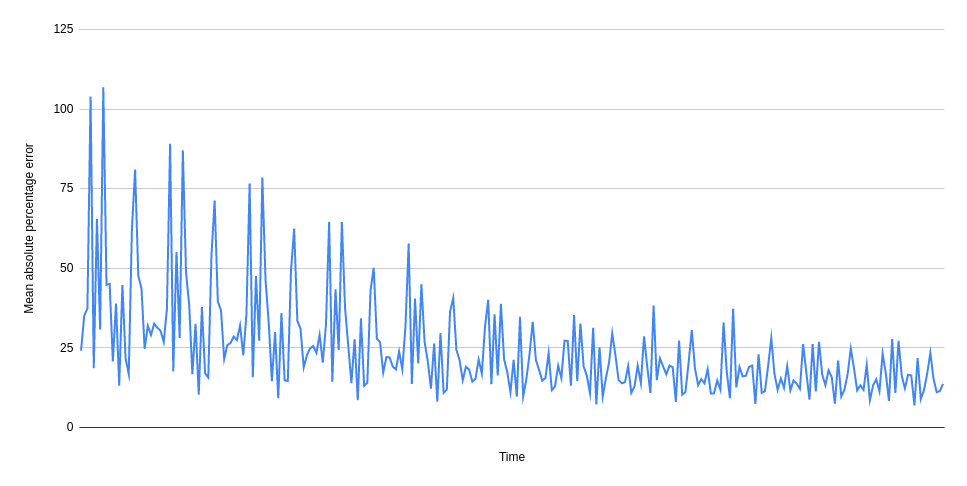
\includegraphics[width=\textwidth]{img/experiment1_results_MeanAbsolutePercentageErrorOverTime.png}
		\caption{...}
	\end{subfigure}
	\caption{...}
	\label{pic:experiment1_results_loss_and_percentageLoss}
\end{figure*}


\section{Lessons Learned}

\filbreak
